\documentclass{bioinfo}

%\usepackage{doi}

\copyrightyear{2014}
\pubyear{2014}

\begin{document}
\firstpage{1}

\title[lossy-compression]{Lossy compression of DNA sequencing quality data}
\author[El Hadidi \textit{et~al.}]{Mohamed El Hadidi\,$^{1}$\footnote{authors contributed equally}, Christopher M. Hill\,$^{2}$\footnotemark[1], Andr\'{a}s Szolek\,$^{3}$\footnotemark[1], and Michael P. Cummings\,$^4$\footnote{to whom correspondence should be addressed}}
\address{$^{1}$Department of Algorithms in Bioinformatics,  Center for Bioinformatics, University of T\"{u}bingen, Sand 14, 72076 T\"{u}bingen, Germany \\
$^{2}$Department of Computer Science, University of Maryland, College Park,  Maryland, 20742 USA\\
$^{3}$Department of Applied Bioinformatics, Center for Bioinformatics, Quantitative Biology Center, and Department of Computer Science, University of T\"{u}bingen, Sand 14, 72076 T\"{u}bingen, Germany\\
$^{4}$Center for Bioinformatics and Computational Biology, University of Maryland, College Park, 20742 USA}
%$\dagger$authors contributed equally
\history{Received on XXXXX; revised on XXXXX; accepted on XXXX}
% Hack to display authors contribution.
\editor{Associate Editor: XXXXXXX}

\maketitle

\begin{abstract}

\section{Motivation:}
The \textsc{fastq} file format has become the \emph{de facto} standard for storing next-generation sequencing data, containing nucleotide information along with a quantitative measure of the reliability of individual base calls.
As the cost of sequencing continues to decrease, the rate of sequencing data production is increasing, requiring efficient ways of storing and transferring this vast amount of data. Most methods on sequencing data compression focus on compressing nucleotide information without any loss of information.
Quality data, however, have different properties than nucleotide data, and methods compressing nucleotide sequences efficiently do not perform as well on quality sequences. Furthermore, while lossless representation is necessary for nucleotide sequences, it is not an essential requirement for quality values.

Existing methods for compressing quality sequences mostly focused on minimizing the loss of information with less emphasis on effects on subsequent analyses. In this paper, we evaluate several different compression methods for quality values that compromise accuracy for better storage efficiency, and their resulting impact on common bioinformatic analyses using sequence read data.

\section{Results:}
Lossy compression of quality information can greatly decrease storage and memory requirements with little discernable effects on subsequent analysis results.
The four compression strategies in this study were able to produce similar results to those obtained with uncompressed quality sequences in terms of quality control, genome assembly, and alignment of short read to a reference sequence.


\section{Contact:} \href{mike@umiacs.umd.edu}{mike@umiacs.umd.edu}
\end{abstract}

\section{Introduction}

The \emph{de facto} standard for storing next-generation sequencing data is the \textsc{fastq} format. A component of \textsc{fastq} format files~\cite{cock2010sanger} is information for a quantitative measure of quality for each nucleotide based on the \textsc{phred} quality value, which is defined as $Q = -10\ log_{10}\/P$~\cite{ewing1998base}. Depending on the sequencing technology these quality values can range from 0 to 93, and the American Standard Code for Information Interchange \textsc{ascii} characters 33 to 126 (with some offset) are used to represent quality values.

Quality values are typically used throughout bioinformatics pipelines.
Certain tools, such as \textsc{fastqc}~\cite{andrews2010fastqc} and Prinseq~\cite{schmieder2011quality}  provide the user with detailed descriptions of the distribution of sequence quality scores. These analyses can then be used to filter and trim the sequencing data~\cite{martin2011cutadapt}.
The processed sequencing data can then be be used in subsequent analyses.
Certain genome assemblers utilize quality values directly to produce better assemblies~\cite{gnerre2011high}. Genome assemblers work by piecing together overlapping sequences, constructing a larger resulting sequence. Short-read alignment tools, such as Bowtie 2~\cite{langmead2012fast}, use quality values to scale the mismatch penalty in a way that mismatches between poor quality bases of the query and the reference are weighted less than mismatches occurring on high quality bases. Similar to alignment, software for detecting single nucleotide polymorphisms (\textsc{snp}s) can also rely on quality values~\cite{mckenna2010genome}. Detected \textsc{snp}s with high-quality bases are more trustworthy than those with low-quality bases, particularly in low coverage regions.

Although the quality values are useful for later steps, the trade-off between storing effectively double the amount of data and the resulting effects on subsequent analyses has not been well-documented. Previous literature on sequence data compression has largely focused on lossless compression of base calls~\cite{sato2001dna,chen2000compression,chen2002dnacompress}. If a reference exists for the biological data, sequences can be compressed using offsets into the reference~\cite{kozanitis2011compressing}. Typical compression methods fail to utilize the biases inherent in existing sequencing technologies. Depending on the sequencing technology used, the base calling is more accurate in the earlier cycles, gradually losing quality in later cycles~\cite{kozanitis2011compressing}.
To this end, methods for compressing these quality sequences utilize these general quality trends. \textsc{SlimGene}~\cite{kozanitis2011compressing} is one such tool that builds a fixed-state Markov model on adjacent quality scores and uses Huffman Coding for compression based on the transition probabilities.

Little prior work has been done examining the effect of lossy compression of quality sequences in the context of subsequent analyses. Our aim here is to examine the effect of multiple lossy compression methods on quality sequences, focusing not only on the differences between the compressed and original versions, but also the effect of lossy compression on typical subsequent analyses.

We examine four general classes of lossy compression methods: score binning, model-based, profile-based, and data type transformation.

One compression strategy is to look at the distribution of quality values and see if we can summarize the information contained within ranges of values. Specifically, we can reduce the dimensionality of the distribution of quality values by binning together adjacent quality values. We can select the number of bins depending on the desired amount of compression and retention of quality information. Taken to nearly the extreme, a base call can be considered either good or bad. This is the motivation of our approach, deemed quality value binning, where we observe the distribution of quality values across the read set and find a cutoff between good and bad bases.

Another compression strategy involves simplifying the data through modeling of the quality values of a given sequence.
By constructing a compact model of our quality values, we only have to store the parameters of the model to recreate the quality sequences.
Intuitively, the simpler the model, the better the compression, but results in potentially higher differences compared to the original quality sequences.
Another benefit of the model-based compression is the ability to decompress any particular quality value in the sequence with constant time during decompression.
In our approach, we represent the quality values of a sequence as a polynomial function, but it is possible to use other models (such as other basis functions or splines).

Profile-based compression utilizes the fact that in a vast set of quality sequences one can identify large classes of highly similar elements. If one could partition the data into such classes, each of those would be efficiently representable with a single consensus profile.

The last approach we investigated is based on transforming the original data into a wholly different representation for which efficient and proven compression algorithms already exist. In this study, we described a way of reducing the problem of quality compression to image compression via blockwise quality data transformation. This approach is different from the others in that depending on the image compression algorithm used it is not restricted to lossy techniques.

\begin{methods}
\section{Methods}

\subsection{Quality value binning}

%The quality value provides some measure of the accuracy of a given base call. A strategy to reduce the dimensionality of these quality values is to aggregate adjacent quality values together into the same bin. Taken to the extreme, a base call can be considered either good or bad. This is the motivation of our approach, deemed good/bad encoding, where we observe the distribution of quality values across the read set and find a cutoff between good and bad bases.

In one of the more extreme cases of quality value binning, we can bin a quality value into one of two categories: good or bad.
We define good/bad encoding as finding the quality value cutoff to separate between good and bad bases.
%The goal of good/bad encoding is to find the quality value cutoff to separate between 
First, we learn the distribution of quality values across all sequences.
Using this distribution, bases are marked bad if their quality value falls below a certain threshold.
We set the cutoff as the first quartile minus 1.5 * the interquartile range (IQR), which is the difference between the first and third quartile.
1.5 * IQR is the value used by Tukey's box plot~\cite{mcgill1978variations}.
The main benefit of this approach is that it is completely data-dependent. No prior assumptions of the distribution of the quality values need to be made.
 
Because we only have two possible choices for a quality of base, this makes a straightforward binary encoding possible, allowing us to use a single bit to represent the quality of a base instead of the default 8 bits used to store quality values in \textsc{ascii}.

Although simple and intuitive, considering a base as either good or bad may be too limiting for some users, so we provide a few additional options to preserve more of the defining characteristics of the quality values, but we only analyze good/bad encoding in our results.

\subsection{Polynomial regression}

One approach to compressing quality values is to treat them as bivariate data with the ordered nucleotides (1 to read length) representing the abscissa, and quality values representing the ordinate. Viewed in this way we can ask the question: is there a mathematical function that describes the relationship between read position and quality value sufficiently, albeit imperfectly (i.e., with some loss of information), such that modeled values perform well in subsequent analyses? 

To this end, we modeled read quality sequences with zero to fifth-degree polynomials obtained with least-squares fitting. However, despite the fact that polynomial functions have significantly lower number of parameters (i.e. one to six coefficients) than a read-length string of raw quality values, the necessity of using floating point numbers to store coefficients greatly limits the compression potential of the method. In order to get meaningful compression on single-precision four-byte floating point numbers, one would have to relax on the least-squares approximation constraint to obtain compressible values on the byte level which is outside the scope of this study.

Nonetheless, fitting a polynomial and reconstructing the quality values that it would have yielded after decompression still makes some sense as it alters the properties of the quality data, making it highly compressible simply due to the smoothing effect it provides. Therefore the compression ratio and bits per bp values for polynomial regression throughout this manuscript refer to bzipped polynomially approximated quality values.

\subsection{Profile-based compression}

As large sets of quality strings show similar trends of quality over their sequence, it makes sense to identify such common patterns in the data and use them as reference profiles to approximate individual quality sequences. Such patterns can be readily determined by clustering data points (i.e. quality vectors) and using the resulting cluster centers as representative profiles.

K-means clustering is a vector quantization method, partitioning a set of samples into K sets that minimize within-cluster sum of squares~\cite{macqueen1967some}. Using a random subset of read quality values, a compression method can use the computed cluster centers as read quality profiles. As the problem is NP-hard, we use a heuristic iterative refinement approach quickly converging to a locally optimal minimum provided by the Python package scikit-learn 0.15~\cite{scikit-learn}.

%First, the method randomly samples from the set of quality sequences to form the training set. The amount of quality sequences sampled can be adjusted by the user.
First, the method samples an adjustable number of quality sequences randomly from the file to be used as a training set. Quality sequences are represented by vectors containing their \textsc{phred} scores corresponding to each position along the read. Subsequently, K-means clustering is performed on the training set until convergence. The obtained cluster centers will be the quality profile prototypes for the dataset.

Once the K quality profiles are determined, all quality sequences are passed through the trained K-means predictor, with the nearest quality profile in Euclidean space being assigned to every quality sequence as their compressed representation.

The compressed quality file therefore consists of an index enumerating the K quality profiles, and a binary part containing the assigned quality profile index for each read.

Although this approach is not able to capture randomly occuring outlier quality values, it ensures that the overall trends in quality sequences are retained. Quality profiles capture different overall qualities and different drop-off positions and gradients. An example of 128 quality profiles are shown on Figure \ref{fig:profiles_128}.

\begin{figure}[!tpb]%figure2
\centerline{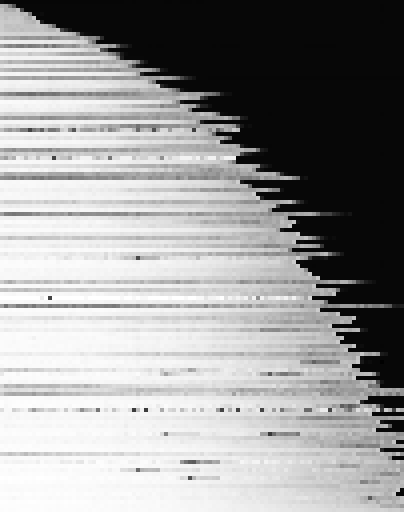
\includegraphics[width=3.35in]{profiles_128.png}}
\caption{Quality profiles obtained by K-means clustering on the fragment library from \textit{Rhodobacter sphaeroides} 2.4.1 data set using K=128, with each row corresponding to a quality profile. Dark to light colors represent low to high quality values. It is readily visible that the two most distinctive features of quality profiles is their drop-off position and average overall quality. One can also see sporadic low-position values in a handful of profiles, likely capturing intermittent problems in the sequencing process affecting thousands of reads at a time.}\label{fig:profiles_128}
\end{figure}


\subsection{Blockwise image compression-based algorithm}

The principle of utilizing image compression algorithms on seemingly dissimilar data such as electromyography signals is not new~\cite{costa2008compression}. Sequence quality values possess some properties such as smooth overall gradients and sudden drop-offs along a sequence whose accurate and efficient representation are crucial to image compression algorithms. Our aim is therefore to reduce the sequencing quality compression problem to a very well known and extensively researched problem, leveraging the power of mature algorithms on the image compression field. The key steps of the problem reduction are:

\begin{enumerate}
    \item Take a number of quality sequences and represent them as a matrix (rows: reads, columns: base positions).
    \item Sort its rows in a way that maximizes smoothness across the matrix, e.g. apply hierarchical clustering, akin to creating a cluster heat map.
    \item Take the resulting matrix as a grayscale image with each pixel's intensity corresponding to the \textsc{phred} score it represents.
    \item Encode the image with a suitable image compression algorithm.
    \item Either store the sorted indices to recover their original order during decompression, or re-order reads corresponding to quality values instead.
\end{enumerate}

\begin{figure*}[!tpb]%figure2
\centerline{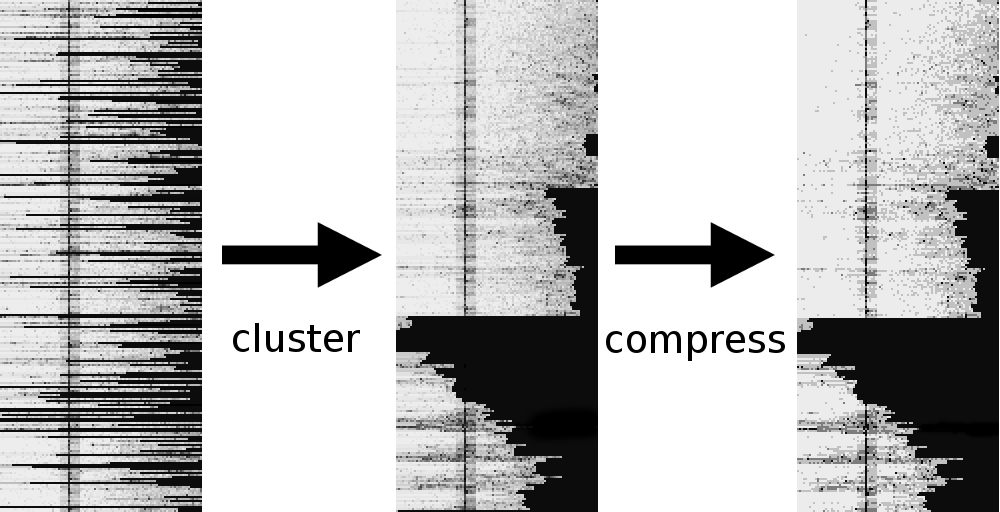
\includegraphics[width=6.9in]{png_pipeline.png}}
\caption{Image compression based approach. Quality values are loaded into a matrix in chunks (256 reads of read-length 101 in the example). Reads are hierarchically clustered, and the rows of the matrix accordingly re-ordered. The new matrix, given its properties such as smoothness and distinct spatial features, lends itself to efficient image compression. Note the uniform dip in quality around position 35: the sequencing process was possibly temporarily compromised, affecting several thousands of reads.}\label{fig:png_method}
\end{figure*}

Lossy image compression algorithms are prone to introducing various artifacts, such as ringing, blockiness, etc. Their implication in this context is unpredictable distortion across multiple positions and even reads. Whether this is an acceptable compromise or not primarily depends on the use case.  In this study, we applied a hybrid approach using lossless Portable Network Graphics (\textsc{png}) encoding on adaptively quantized data, all performed by the \textsc{png} encoder pngquant 2.3.0 (http://pngquant.org/). This method is free of the previously mentioned artifacts, and provides an adjustable level of compression.

The choice of this particular image encoder is not essential to the algorithm, but rather serves as an initial proof of concept implementation. Other image compression algorithms could be explored extensively, and seamlessly substituted into our method for further benchmarking.

Our method uses mean linkage hierarchical clustering for row sorting, which, just like the image encoder, can be replaced with other linkage criteria or even sorting methods to be evaluated for performance.

\subsection{Data sets}

For our analyses, we use sequencing data provided by the \textsc{GAGE} project~\cite{salzberg2012gage}.
The read data for \textit{Rhodobacter sphaeroides} 2.4.1 was downloaded from
\href{http://gage.cbcb.umd.edu/data/Rhodobacter_sphaeroides}{http://gage.cbcb.umd.edu/data/Rhodobacter\_sphaeroides},
%http://gage.cbcb.umd.edu/data/Rhodobacter\_sphaeroides
and the corresponding reference sequence was obtained from the NCBI RefSeq database (NC\_007488.1, NC\_007489.1, NC\_007490.1, NC\_007493.1, NC\_007494.1, NC\_009007.1, NC\_009008.1).
The \textit{Rhodobacter sphaeroides} 2.4.1 data set consists of 2,050,868 paired-end reads (insert size of 180 bp) and 2,050,868 short-jump reads (insert size of 3,000 bp).


%\begin{table}[!t]
%\processtable{This is table caption\label{Tab:01}}
%{\begin{tabular}{llll}\toprule
%head1 & head2 & head3 & head4\\\midrule
%row1 & row1 & row1 & row1\\
%row2 & row2 & row2 & row2\\
%row3 & row3 & row3 & row3\\
%row4 & row4 & row4 & row4\\\botrule
%\end{tabular}}{This is a footnote}
%\end{table}

\subsection{Evaluating lossy compression algorithms}


Lossy compression compromises representation accuracy for better space efficiency. Different lossy compression methods have different properties, therefore we need to evaluate a number of tradeoffs for each of our proposed methods. More importantly, we need to examine each approach in the context of typical bioinformatics tasks, such as quality control, \emph{de novo} genome assembly, and aligning the sequences to a given reference.

For quality control, we use Autoadapt tool which uses \textsc{fastqc}~\cite{andrews2010fastqc} and \textsc{CutAdapt}~\cite{martin2011cutadapt} packages with the default settings. PrinSeq~\cite{schmieder2011quality} was used to count the number of bases and reads in each \textsc{fastq} file.

For \emph{de novo} genome assembly, we use \textsc{allpaths-lg}~\cite{gnerre2011high} version r50191 with default settings and 32 threads.

For aligning the sequences, we use Bowtie 2~\cite{langmead2012fast} with default settings and modified max- and min-mismatch parameters detailed below.

\end{methods}

\section{Results}

\subsection{Compressibility}

For any lossy compression method, we need to evaluate the tradeoff between its physical compression and the loss in its accuracy.
Here, we use average \emph{bits per bp} to measure the physical compression of the data and mean squared error (MSE) to measure the loss in quality.
Bits per bp is calculated simply as the compressed file size (in bits) divided by the total number of quality values.
MSE is calculated by $\frac{1}{n}\sum_{i=1}^{n}{(Q_i-Q_i')^2}$, where $n$ is the number of sequences, $Q_i$ is the actual quality value associated with sequence position $i$, and $Q_i'$ is the corresponding compressed quality value.

We compare the \textsc{mse} versus \emph{bits per bp} of the fragment and short-jump libraries of the  \textit{Rhodobacter sphaeroides} 2.4.1 data set (Figures \ref{fig:mse_vs_bpbp_frag} and \ref{fig:mse_vs_bpbp_jump}). Storing the uncompressed quality values requires 1 \emph{byte} per basepair because they are stored in \textsc{ascii} format; however, losslessly compressing the values with BZip2 2.112 bits per basepair. 0-order polynomial regression and 32-profile encodings have the lowest bits per bp. 5th-order polynomial regression and \textsc{png} encodings have the highest bits per bp, but have among the lowest \textsc{mse}. Despite having similar bits per bp, \textsc{png} encoding has roughly one third the \textsc{mse} as 5th-order polynomial (3.07 vs 10.27, respectively).

As the order of the polynomial increases, the bits per bp increase and the \textsc{mse} decreases at an exponential rate.

\begin{figure}[!tpb]%figure2
\centerline{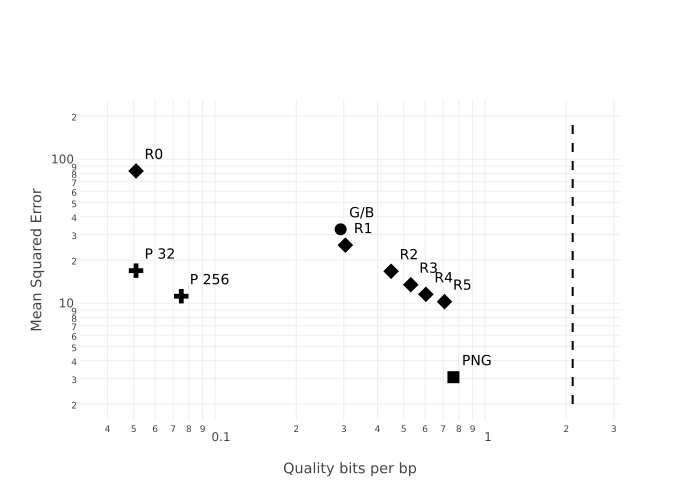
\includegraphics[width=3.65in]{mse_frag.png}}
\caption{MSE versus bits per bp for different compression methods applied to the fragment library from \textit{Rhodobacter sphaeroides} 2.4.1 data set. G/B: Good/Bad encoding. P32 and P256: Quality profile compression with 32 and 256 profiles. R0-R5: Polynomial regression-based compression using 0-5 degrees. PNG: Blockwise image compres the generated SAM file for each compressing approach weresion algorithm. Dashed line corresponds to lossless bzip compression of quality values. \em}\label{fig:mse_vs_bpbp_frag}
\end{figure}

\begin{figure}[!tpb]%figure2
\centerline{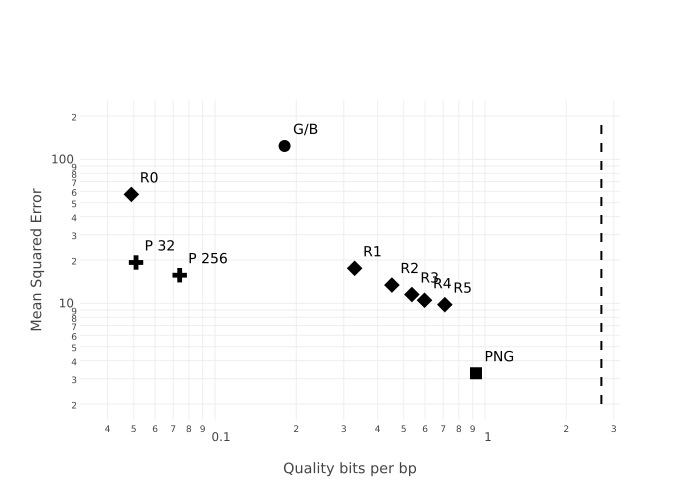
\includegraphics[width=3.65in]{mse_short.png}}
\caption{MSE versus bits per bp for for different compression methods applied to the short-jump library from \textit{Rhodobacter sphaeroides} 2.4.1 data set. G/B: Good/Bad encoding. P32 and P256: Quality profile compression with 32 and 256 profiles. R0-R5: Polynomial regression-based compression using 0-5 degrees. PNG: Blockwise image compression algorithm. Dashed line corresponds to lossless bzip compression of quality values. \em}\label{fig:mse_vs_bpbp_jump}
\end{figure}

\subsection{Lossy compression effect on preprocessing quality}

One way to evaluate different compression approaches is to perform quality preprocessing on the generated \textsc{fastq} files and compare the number of reads and bases with those of the uncompressed \textsc{fastq} files.
Autoadapt is a tool that uses \textsc{fastqc} and \textsc{Cutadapt}  to filter and trim reads.
We used PrinSeq to calculate the number of reads and bases in each sample. Table \ref{tab:quality_control} shows the proportional numbers with respect to those of the uncompressed \textsc{fastq} files.
In the fragment sample, we retain on average 95.4\% and 94.24\%  of bases and reads, respectively. In the short-jump sample, we retain 90.4\% and 90.98\% of bases and reads, respectively. In some cases, the proportion of reads and/or bases compared to the original is more than 100\%; this means that the number of the reads and bases in the compressed samples are more because altering quality values may prevent the read from being filtered and/or trimmed. This is clear in the good/ bad compression approach of the short-jump sample, where the proportion of bases and reads are 113.09\%  and 103.70\% respectively.


\subsection{Lossy compression effect on assembly quality}


Genome assemblers, such as \textsc{allpaths-lg}~\cite{gnerre2011high}, often utilize quality values to aid in the assembly process. By reducing the information contained within the quality values, we introduce the potential for the resulting assembly to be affected.

\textsc{allpaths-lg} is one of the leading bacterial genome assemblers~\cite{salzberg2012gage}. We examine the effect of our lossy compression methods on the \textit{Rhodobacter sphaeroides} 2.4.1 data set provided by \textsc{gage} (Genome Assembly Gold-Standard Evaluations)~\cite{salzberg2012gage}. \textsc{allpaths-lg} is used to assemble the original data along with the quality compressed versions using good/bad encoding, 0--5th-order polynomial regression encodings, 32- and 256-profile encodings, and \textsc{png} encoding. We evaluate the assembly based on contiguity statistics, log average read probability (LAP~\cite{ghodsi2013novo}), and a collection of reference-based metrics. The contiguity statistics include number of scaffolds and NG50, which is defined as the weighted median contig size (the length of largest contig $c$ such that the total size of the contigs larger than $c$ exceeds half of the known genome size).  The LAP score can be viewed as a log likelihood score, where a value closer to 0 is better. We use a reference-based evaluation script provided by \textsc{gage} which counts single nucleotide polymorphisms (\textsc{snp}s), relocations, translations, and inversions. The reference-based metrics are normalized by the length of the assembly to aid in comparison. Alongside the raw metrics, we also provide a cummulative sum of the individual ranks of each method for each metric. A similar approach was utilized by the \textsc{Assemblathon1} competition~\cite{earl2011assemblathon}.


The assembly using the uncompressed reads outperforms all compression methods in terms of LAP, NG50, relocations, translations, and inversions (Table \ref{tab:assembly_ranks}). Among the compression methods, the \textsc{png} encoding had the highest rank, followed by 256- and 32-profile encoding, then the 4th-order polynomial regression, the 5th-order polynomial regression, the good/bad encoding, and lastly, the 3rd through 0-order polynomials.

The lossy compression methods largely preserve the contiguity found in the assembly produced using the reads with unmodified quality sequences. All compression methods other than 0-order polynomial regression produce an NG50 ranging from 3.18--3.19 Mbps. Despite the similar contiguity statistics, the different compression methods vary noticeably in the amount of SNPs. The order of polynomial has an inverse relationship with the amount of SNPs detected.
The good/bad, profile and PNG methods detected the least amount of SNPs compared to the reference genome, outperforming the assembly using the original quality sequences.
A more indepth evaulation is needed to determine whether these compression methods are missing actual SNPs.

It is important to highlight the result that the 4th-order polynomial regression outperforms the 5th-order in all of the reference-based metrics, but not the \emph{de novo} LAP metrics. The 5th-order polynomial regression assembles approximately 2.5 kb more sequence and uses roughly $1.2\%$ more of the total read set than the 4th-order (Supplemental Table 1), which may explain the discrepency in LAP values because the LAP value is influenced by total coverage~\cite{ghodsi2013novo}.


\begin{table*}[!tpb]
%\processtable{Rankings of different assemblies created using proposed compression methods. Assemblies were created using \textsc{allpaths-lg} and the \textit{Rhodobacter sphaeroides} 2.4.1. data set provided by \textsc{gage}\citep{salzberg2012gage}.\label{tab:assembly_ranks}}
\centering
\caption[]{Rankings of different assemblies produced using proposed compression methods. Assemblies were constructed using \textsc{allpaths-lg} and the \textit{Rhodobacter sphaeroides} 2.4.1. data set provided by \textsc{gage}~\cite{salzberg2012gage}. Regression methods are sorted by their overall rank (determined by the sum of individual rankings).}
{\begin{tabular}{lcccccccc}
& Overall & & & & & & LAP & LAP \\
Compression            & rank & \textsc{snp}s & Inversions & Relocations & Translocations & Indels & fragment & short-jump \\
\hline
None                   & 1    & 5    & 1          & 1           & 1              & 1      & 1          & 1                    \\
PNG                    & 2    & 4    & 1          & 2           & 2              & 3      & 4          & 2                    \\
Profile (256)          & 3    & 2    & 1          & 3           & 3              & 4      & 2          & 4                    \\
Profile (32)           & 4    & 3    & 1          & 4           & 6              & 5      & 3          & 3                    \\
Regression (4th order) & 5    & 6    & 1          & 6           & 5              & 2      & 7          & 8                    \\
Regression (5th order) & 6    & 7    & 1          & 5           & 7              & 7      & 5          & 7                    \\
Good/bad               & 7    & 1    & 1          & 8           & 11             & 10     & 6          & 5                    \\
Regression (3rd order) & 8    & 8    & 1          & 9           & 9              & 6      & 8          & 6                    \\
Regression (2nd order) & 9    & 9    & 1          & 7           & 4              & 8      & 9          & 10                   \\
Regression (1st order) & 10   & 10   & 11         & 10          & 8              & 9      & 10         & 9                    \\
Regression (0 order) & 11   & 11   & 10         & 11          & 10             & 11     & 11         & 11
\\ \hline
\end{tabular}
}
\label{tab:assembly_ranks}
\end{table*}

\subsection{Lossy compression effect on mapping quality}

Certain short read alignment tools use the quality sequence information when finding potential alignments. Bowtie 2 (version 2.2.3) was used to evaluate the different decompressed \textsc{fastq} files. Bowtie 2 uses quality values written in the \textsc{fastq} files when mapping reads against a reference genome. The original uncompressed and decompressed \textsc{fastq} files were mapped with Bowtie 2 against \textit{Rhodobacter sphaeroides} reference genome. The generated \textsc{sam} file for each compressing approach were compared with the uncompressed \textsc{sam} file. The total, shared and unique proportional numbers of mapped reads are calculated with respect to the uncompressed \textsc{sam} matches as shown in table \ref{tab:aligner}. Additionally, to monitor the effect of quality values on mapping in general, Bowtie 2 was tweaked with the maximum and minimum mismatch penalty equivalent to maximum and minimum quality scores (with parameters: --mp 6,6 and --mp 2,2 respectively).

Generally, increasing the regression model polynomial order from 0 to 5 results in more mapped reads with the most marked change from order 1 to order 2. The best compression approach is the one that has highest proportion of reads shared between the uncompressed and decompressed files and least number of reads that are unique in both uncompressed and decompressed files. In fragment sample, on average, 99.03\% of reads were mapped using different compression approaches, within which 99\% are shared with the uncompressed alignments and 0.02\% unique mapped reads in the decompressed file. The average missed alignments are 0.99\%. Compression with profile 256 approach was shown to be the best performing approach in the fragment decompressed sample, as a proportional of 99.94\% reads are mapped with respect to the uncompressed mapped reads within which 99.91\% are common and only 0.08\% unique mapped reads in the decompressed file. In short-run sample, the average number of mapped reads is 99.14 \% within which 98.73\% are common and 0.41\% unique mapped reads in the decompressed file.The average missed alignments are 1.2\%. Regression with the 5th polynomial order captured the highest mapped reads of 100\%, within which 99.66\% are common and only 0.33\% unique mapped reads in the decompressed file. In both samples, \textsc{png} compression has the least number of mapped reads that are unique in the decompressed files (only  0.013\% and 0.89\% in the fragments and short-jump samples, respectively).



\begin{table*}[!tbhp]
\centering
\caption[]{Mapping results of decompressed \textsc{fastq} files against \textit{Rhodobacter sphaeroides} reference genome using Bowtie 2. Numbers corresponds to the proportion of mapped reads with respect to the uncompressed \textsc{fastq}. ``Shared'' denotes the percentage of mapped reads by both the uncompressed and decompressed data. ``Uncompressed only'' denotes the percentage of reads mapped from the uncompressed data that are not mapped after decompression. ``Compressed only'' denotes the percentage of reads mapped from the decompressed data that were not mapped before compression.}
\begin{tabular}{llcccc}
    & & \multicolumn{4}{c}{Percentage of reads mapped}\\
    \cline{3-6}
	Library & Compression Strategy & Total & Shared & Uncompressed only & Compressed only \\ \hline
	& Maximum quality & 77.88 & 77.88 & 22.12 & 0 \\
	&Minimum quality & 100 & 100 & 0 & 0 \\
	&Good/Bad & 99.92 & 99.89 & 0.11 & 0.03 \\
	&Regression (0 order) & 93.63 & 93.62 & 6.38 & 0.02 \\
	&Regression (1st order) & 98.62 & 98.61 & 1.39 & 0.01 \\
	&Regression (2nd order) & 99.42 & 99.39 & 0.61 & 0.03 \\
	Fragment&Regression (3rd order) & 99.56 & 99.53 & 0.47 & 0.03 \\
	&Regression (4th order) & 99.71 & 99.68 & 0.32 & 0.03 \\ 
	&Regression (5th order) & 99.79 & 99.75 & 0.25 & 0.03 \\
	&Profile (32) & 99.9 & 99.86 & 0.14 & 0.04 \\ 
	&Profile (256) & 99.95 & 99.92 & 0.08 & 0.03 \\
	&PNG & 99.82 & 99.81 & 0.19 & 0.01 \\ 

\\ \hline \\

	&Maximum quality & 78.08 & 78.08 & 21.92 & 0 \\
	&Minimum quality & 100 & 100 & 0 & 0 \\ 
	&Good/Bad & 97.38 & 97.38 & 2.62 & 0 \\
	&Regression (0 order) & 96.07 & 94.11 & 5.89 & 1.96 \\
	&Regression (1st order) & 99.24 & 98.98 & 1.02 & 0.26 \\ 
	&Regression (2nd order) & 99.66 & 99.35 & 0.65 & 0.3 \\ 
	Short-jump&Regression (3rd order) & 99.94 & 99.61 & 0.39 & 0.33 \\ 
	&Regression (4th order) & 99.99 & 99.64 & 0.36 & 0.35 \\ 
	&Regression (5th order) & 100 & 99.67 & 0.33 & 0.33 \\ 
	&Profile (32) & 99.74 & 99.44 & 0.56 & 0.3 \\
	&Profile (256) & 99.76 & 99.52 & 0.48 & 0.24 \\
	&PNG & 99.71 & 99.62 & 0.38 & 0.09 \\ \hline
\end{tabular}

\label{tab:aligner}
\end{table*}


\begin{table}[!tbhp]
\centering
\caption[]{Quality filtering/trimming for the uncompressed and decompressed \textsc{fastq} files. Numbers correspond to the proportion of bases/reads that are missed or gained after applying compression with respect to the uncompressed values.}
\label{tab:quality_control}
\begin{tabular}{lcccc}
	 & \multicolumn{2}{c}{Fragments} & \multicolumn{2}{c}{Short-Jump} \\
	 & \% Bases & \% Reads & \% Bases & \% Reads \\ \hline
	Good/bad & 98.15 & 98.78 & 113.09 & 103.7 \\ 
	Regression (0 order) & 86.71 & 62.64 & 43.31 & 27.51 \\
	Regression (1st order) & 92.96 & 95.09 & 81.31 & 91.79 \\ 
	Regression (2nd order) & 93.93 & 96.87 & 86.31 & 94.75 \\
	Regression (3rd order) & 93.5 & 95.68 & 88.7 & 94.51 \\ 
	Regression (4th order) & 94.43 & 96.7 & 91.94 & 97.02 \\ 
	Regression (5th order) & 95.56 & 98.09 & 93.92 & 98.02 \\ 
	Profile (32) & 99.12 & 98.96 & 102.89 & 102.24 \\
	Profile (256) & 100 & 99.8 & 102.66 & 101.27 \\
	PNG & 99.62 & 99.75 & 99.84 & 99 \\ \hline
\end{tabular}
\end{table}

\section{Discussion}

\subsection{Lossy compression acceptable for subsequent biological analyses}

The primary concern of using lossy compression methods is naturally the extent of information loss, that we quantified by \textsc{mse} in this study. \textsc{mse} and compressibility provide information in the theoretical context to the methods, but they are not the end-all of evaluation criteria. The performance of compressed datasets in different subsequent analyses and applications are just as important. Our benchmarks showed that some of the compression methods with high error rates are still practical for certain kinds of applications. Many subsequent tools proved to have enough additional redundancy built-in to handle such loss in information.
Passing the decompressed quality sequences through quality control software shows that most methods filter nearly as many bases as using original quality sequences.
Assemblers performing sequencing alignment use percent similarity scores that are typically robust to standard sequencing errors. 


\subsection{Extension of good/bad encoding}


Good/bad encoding has the nice property of being simple to compute and has a good bits per bp score. The good/bad encoding suffers from having a high \textsc{mse}, but fortunately, we have shown that in the case of genome assembly, good/bad encoding outperforms all polynomial regressions encodings with degree less than 3. Good/bad encoding of the fragment and short-jump libraries of \textit{Rhodobacter sphaeroides} have \textsc{mse}s of $2.42\times$ and $10.76\times$ the 3rd-order polynomial regression encodings, respectively. This further highlights the importance of using additional contextual information of the subsequent analyses when evaluating compressed quality values.

A potential extension to good/bad encoding is to incorporate an additional value \emph{okay}.  The \emph{okay} value can be used where the base qualities fall within a good/bad range. Because the distribution of quality values is skewed towards higher quality, we need to experiment with different cutoffs for the \emph{okay} value and determine if the additional storage is noticeable in subsequent analyses.

\subsection{Potential for operations on compressed data}

Perhaps one of the greatest benefits of compressing quality values is the potential to perform quality control and possibly other operations directly on the compressed representations of the data. The tool \textsc{CutAdapt} trims reads that contains a given number of low quality bases from the ends and discards reads that are below a certain threshold. It is trivial to apply the same rules to a few of our compressed quality sequences. In the good/bad encoding, we store a single bit for each quality value. A read with stretches of 0-bits towards the ends can be trimmed and filtered if there are more 0-bits than 1-bits.

In principle, we can quality filter the polynomial regression compression by interpolating where the polynomials are below a certain threshold and then filtering/trimming that part of the read. Unfortunately, storing the coefficients of the polynomials as a float leads to very poor compression.

A beneficial feature of the profile-based approach is that read quality filtering and/or trimming can be performed on the fly during decompression at virtually no computational cost. As all reads are classified into one of $K$ quality profiles, we can determine which of these profiles are of use for subsequent processes, and only decompress reads assigned to these profiles. Furthermore, it is possible to determine trimming points for each profile before extraction, that can be carried out on-line on reads during decompression.

\subsection{The economics of lossy quality sequence compression}

From an economics perspective, we can examine the fixed and marginal costs associated with our lossy compression techniques with respect to memory and computation.
For our quality value binning, modeling-based, and image-based compression methods there are no explicit fixed costs in terms of memory, unlike the profile--based approach, which has a small fixed cost in storing the profiles.
However, the profile-based approach has a much smaller marginal compared to the rest due to the fact that we are simply storing the profile index for each quality sequence.

Regarding computational costs, only quality binning and the profile--based methods have associated fixed costs.
Before performing compression, we have to determine the optimal thresholding values for quality binning, and the cluster representatives for the profile--based method.

In practice, the specific values of these costs are very sensitive to the implementation details.

\subsection{Future of lossy compression in bioinformatics analyses}

We have simply provided here the initial steps in analyzing the effect of lossy compression on quality sequences using a single, high-coverage bacterial data set. More work needs to be done using additional biological data sets, such as human and mouse, along with different sequencing technologies.
A more direct comparison against related lossy compression tools, such as \textsc{SlimGene}~\cite{kozanitis2011compressing} and \textsc{QualComp}~\cite{ochoa2013qualcomp}, needs to be performed. Additionally, other types of sequencing data can be analyzed apart from the Illumina data examined here. For example, the PacBio sequencing instruments produce very long reads (with average read lengths on the order of 10 kbp), but with the trade-off of having a high error-rate ($\sim$15\%).
Unlike the class of quality values we have examined here, the distribution of erroneous bases is relatively uniform~\cite{ferrarini2013evaluation}.
Koren et al.~\cite{koren2013reducing} have shown that the assembly complexity of bacterial genomes can be greatly simplified, producing near complete genome assemblies, by utilizing a single run of these long reads.
If long read sequencing technologies such as PacBio become more widely adopted, it would be of huge benefit to examine the potential of lossy compression algorithms on not only the quality values, but the biological sequencing data themselves.


%%%%%%%%%%%%%%%%%%%%%%%%%%%%%%%%%%%%%%%%%%%%%%%%%%%%%%%%%%%%%%%%%%%%%%%%%%%%%%%%%%%%%
%
%     please remove the " % " symbol from \centerline{\includegraphics{fig01.eps}}
%     as it may ignore the figures.
%
%%%%%%%%%%%%%%%%%%%%%%%%%%%%%%%%%%%%%%%%%%%%%%%%%%%%%%%%%%%%%%%%%%%%%%%%%%%%%%%%%%%%%%




\section{Conclusion}

In this paper we have examined lossy compression on sequence quality values and their effect on subsequent analyses. Although most previous examinations on lossy compression primarily focused on information loss, we have shown that typically used bioinformatics software today have additional built-in sensitivity to handle significant loss of information in the compressed quality values.


\section*{Acknowledgement}
We thank the organizers and participants of the 2014 University of T\"{u}bingen and University of Maryland Bioinformatics Exchange for Students and Teachers (BEST) Summer School.

%\bibliographystyle{natbib}
%\bibliographystyle{achemnat}
%\bibliographystyle{plainnat}
%\bibliographystyle{abbrv}
%\bibliographystyle{bioinformatics}
%
\bibliographystyle{plain}
%
\bibliography{Compression}


\end{document}